% ---------------------------------------------------------------------------
% General proof that K(2k+n, k), n > 0, is not CFON* 1-colorable.
% Written up from handwritten notes (pages 1, 2 and 7). The wording has been
% edited for grammar and clarity; every step of the notes is kept.
% Changes to the mathematics or notation of the notes are marked with a
% comment beginning "% CHANGED:" on the line above them.
% ---------------------------------------------------------------------------
\documentclass[11pt]{article}
\usepackage[margin=1in]{geometry}
\usepackage{amsmath,amssymb}
\usepackage{blkarray}
\usepackage{tikz}
\setlength{\parindent}{0pt}
\setlength{\parskip}{0.8em}

\title{Kneser graphs $K(2k+n,\,k)$ with $n>0$ are not CFON$^{*}$ 1-colorable:\\[2pt]
       the general proof}
\author{Shrey Shah}
\date{}

\begin{document}
\maketitle

\section{Efficient open dominating sets and CFON$^{*}$ 1-colorings}

% CHANGED: "efficient dominating set" in the notes is written "efficient open
% dominating set" throughout.
An efficient open dominating set of a Kneser graph $K$ is a subset $T$ of the
vertices of $K$ such that every vertex of $K$ has \underline{exactly} one
neighbor in $T$.

% CHANGED: the notes leave this sentence unfinished ("because if T is the set
% of all colored vertices"); the conclusion of the "if" is written out.
Note that an efficient open dominating set is analogous to a CFON$^{*}$
1-coloring: if $T$ is the set of all colored vertices, then the coloring is
valid exactly when every vertex has exactly one neighbor in $T$ (since we only
have one color, we can treat all colored vertices as the same).

Assign each vertex $v$ of $K$ a variable:
\[
  x_v =
  \begin{cases}
    1, & v \in T\\
    0, & v \notin T
  \end{cases}
\]

Thus, for every vertex $v$, the variables of the vertices in its open
neighborhood $N(v)$ sum to 1.

\section{The matrix equation}

So for every vertex $v$, summing over the vertices $u$ in $N(v)$:
% CHANGED: ||N(v)|| -> |N(v)| (cardinality).
\[
  \sum_{u \in N(v)} x_u
  \;=\; \underbrace{0 + 0 + 0 + \cdots}_{|N(v)|-1}
  \;+\; \underbrace{1}_{\text{the colored vertex}}
  \;=\; 1
\]

Let $A$ be a matrix in which each row and each column represents a vertex. Let
an element equal 1 if the vertices of its row and column are adjacent, and 0
otherwise.

% CHANGED: the handwritten drawing has an extra edge b--f that is not in the
% matrix. The figure below is drawn to match the matrix (a 5-cycle).
Example:\quad
\begin{minipage}{0.36\textwidth}
\centering
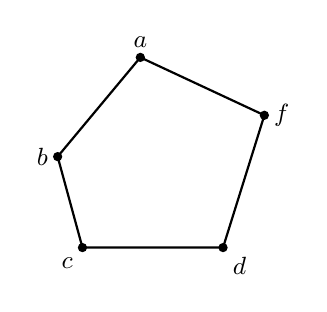
\begin{tikzpicture}[scale=1.05, every node/.style={font=\small}]
  \coordinate (a) at (1.0,2.3);
  \coordinate (f) at (2.5,1.6);
  \coordinate (b) at (0.0,1.1);
  \coordinate (c) at (0.3,0.0);
  \coordinate (d) at (2.0,0.0);
  \draw[thick] (a)--(b)--(c)--(d)--(f)--(a);
  \foreach \p in {a,b,c,d,f} \fill (\p) circle (1.6pt);
  \node[above]       at (a) {$a$};
  \node[left]        at (b) {$b$};
  \node[below left]  at (c) {$c$};
  \node[below right] at (d) {$d$};
  \node[right]       at (f) {$f$};
\end{tikzpicture}
\end{minipage}
\begin{minipage}{0.5\textwidth}
\[
  \begin{blockarray}{cccccc}
      & a & b & c & d & f \\
    \begin{block}{c[ccccc]}
      a & 0 & 1 & 0 & 0 & 1 \\
      b & 1 & 0 & 1 & 0 & 0 \\
      c & 0 & 1 & 0 & 1 & 0 \\
      d & 0 & 0 & 1 & 0 & 1 \\
      f & 1 & 0 & 0 & 1 & 0 \\
    \end{block}
  \end{blockarray}
\]
\end{minipage}

% CHANGED: ||K|| -> |V(K)| (number of vertices of K).
Let $x$ be a $|V(K)| \times 1$ matrix (a vector) in which each element
represents a vertex. Let an element equal 1 if the corresponding vertex is
colored, and 0 otherwise.

% CHANGED: the last entry of the vector was written x_c; it is x_f, the last
% vertex of the example.
\[
  Ax \;=\; A
  \begin{bmatrix} x_a \\ x_b \\ \vdots \\ x_f \end{bmatrix}
  \;=\;
  \begin{bmatrix} 1 \\ 1 \\ \vdots \\ 1 \end{bmatrix}
  \;\longleftarrow\;
  \parbox{0.4\textwidth}{\raggedright the number of colored vertices in the
  neighborhood of the corresponding vertex}
\]

% CHANGED: sentence added. The notes write this vector as a plain "1" on the
% later pages; it is written \mathbf{1} so it is not confused with the number 1.
The all-ones vector on the right is written $\mathbf{1}$ from here on.

\section{The general case $K(2k+n,\,k)$}

We generalize to $K(2k+n,\,k)$ with $k \ge 1$ and $n > 0$.

The graph is $\dbinom{k+n}{k}$-regular.

Let $M$ be its adjacency matrix: each row and each column corresponds to a
vertex, and an element equals 1 if the vertices of its row and column are
adjacent, and 0 otherwise. Each row of $M$ has $\dbinom{k+n}{k}$ 1's.

Consider the equation $Mq = \mathbf{1}$, and suppose every element of $q$ is
the same constant $g$:
\[
  q = \begin{bmatrix} g \\ g \\ \vdots \\ g \end{bmatrix}
\]

% CHANGED: the notes have ((k+n)!/k!) g = 1 and g = k!/(k+n)!. The degree is
% the binomial coefficient (k+n)!/(k! n!), so the n! is restored.
Then each row gives
\[
  \left( \frac{(k+n)!}{k!\,n!} \right) g = 1,
  \qquad
  g = \frac{k!\,n!}{(k+n)!}
\]

The eigenvalues of $M$ are
\[
  \lambda_j = (-1)^j \binom{k+n-j}{k-j}, \qquad j = 0, 1, 2, \dots, k
\]

% CHANGED: the notes say the magnitude is never 0 "because n is strictly
% greater than 0". The eigenvalues are nonzero for every n >= 0; what n > 0
% gives is degree >= 2, i.e. fractional entries of q. The reason is corrected
% here and the n > 0 clause is moved below, to where it is used.
Their magnitudes are never 0, because $k+n-j \ge k-j \ge 0$ for every $j$,
which makes every $\dbinom{k+n-j}{k-j}$ at least 1. Thus every eigenvalue of
$M$ is non-zero, making $M$ invertible.

% CHANGED: the notes say "Using the same invertibility argument as before, q
% is the unique solution, and all its elements are fractional, so no
% efficient open dominating set exists." The argument referred to is written
% out below for M and q, following the notes' argument for K(2k+1,k), so that
% this file stands on its own. N_0^n is written N_0^{|V(K)|} so the exponent
% does not collide with the n of K(2k+n,k).
Now suppose there were some vector $w \in \mathbb{N}_0^{|V(K)|}$ with
$Mw = \mathbf{1}$, so that $w$ meets the CFON$^{*}$ coloring restrictions.

Then:
\begin{align*}
  Mw &= Mq = \mathbf{1} \\
  M^{-1}Mw &= M^{-1}Mq && \text{(since $M$ is invertible)} \\
  w &= q
\end{align*}
But $q$ is fractional: $n$ is strictly greater than 0, which makes
$\dbinom{k+n}{k} \ge k+1 \ge 2$, and so $0 < g < 1$. This contradicts the
definition of $w$. Thus $w$ cannot exist, and $q$ is the unique solution.

Since $q$ is the unique solution and all its elements are fractional, while
each $x_v$ can only equal 0 or 1 depending on whether $v$ is in $T$, no
efficient open dominating set exists, and thus $K(2k+n,\,k)$ is not
CFON$^{*}$ 1-colorable.

\end{document}
